\providecommand{\main}{../../../..}
\documentclass[\main/dresen_thesis.tex]{subfiles}

\begin{document}
  The solvent and co-solvent of the dispersion for the drop casting experiment determine the mobility of the nanoparticles and the time scales for the drop casting experiment.
  Early studies on drop casting of dodecanethiol-ligated gold nanospheres show that a combination of a toluene, a quickly evaporating solvent, as primary dispersion medium and dodecanethiol, a solvent with high-boiling point, as co-solvent results in long-range ordered nanostructure with spheres aligned on an hexagonal lattice \cite{Bigioni_2006_Kinet}.
  This idea has been transferred to oleic acid-ligated ferrite nanoparticles.
  The influence of the choice of primary/co-solvent mixture is studied by performing drop casting experiments using the nanocubes Ol-CoFe-C with varied alkane/alkene combinations.
  As alkane, n-pentane, n-hexane and n-heptane are chosen as rapidly evaporating component and for the high-boiling point alkene, 1-octadecene, 1-hexadecene, 1-dodecene, 1-decene and 1-tetradecene are studied.
  For every experiment the nanoparticle concentration of the dispersion is set to $0.13 \unit{mg/mL}$ and the co-solvent concentration to $2\unit{\%}$.

  \begin{figure}[tb]
    \centering
    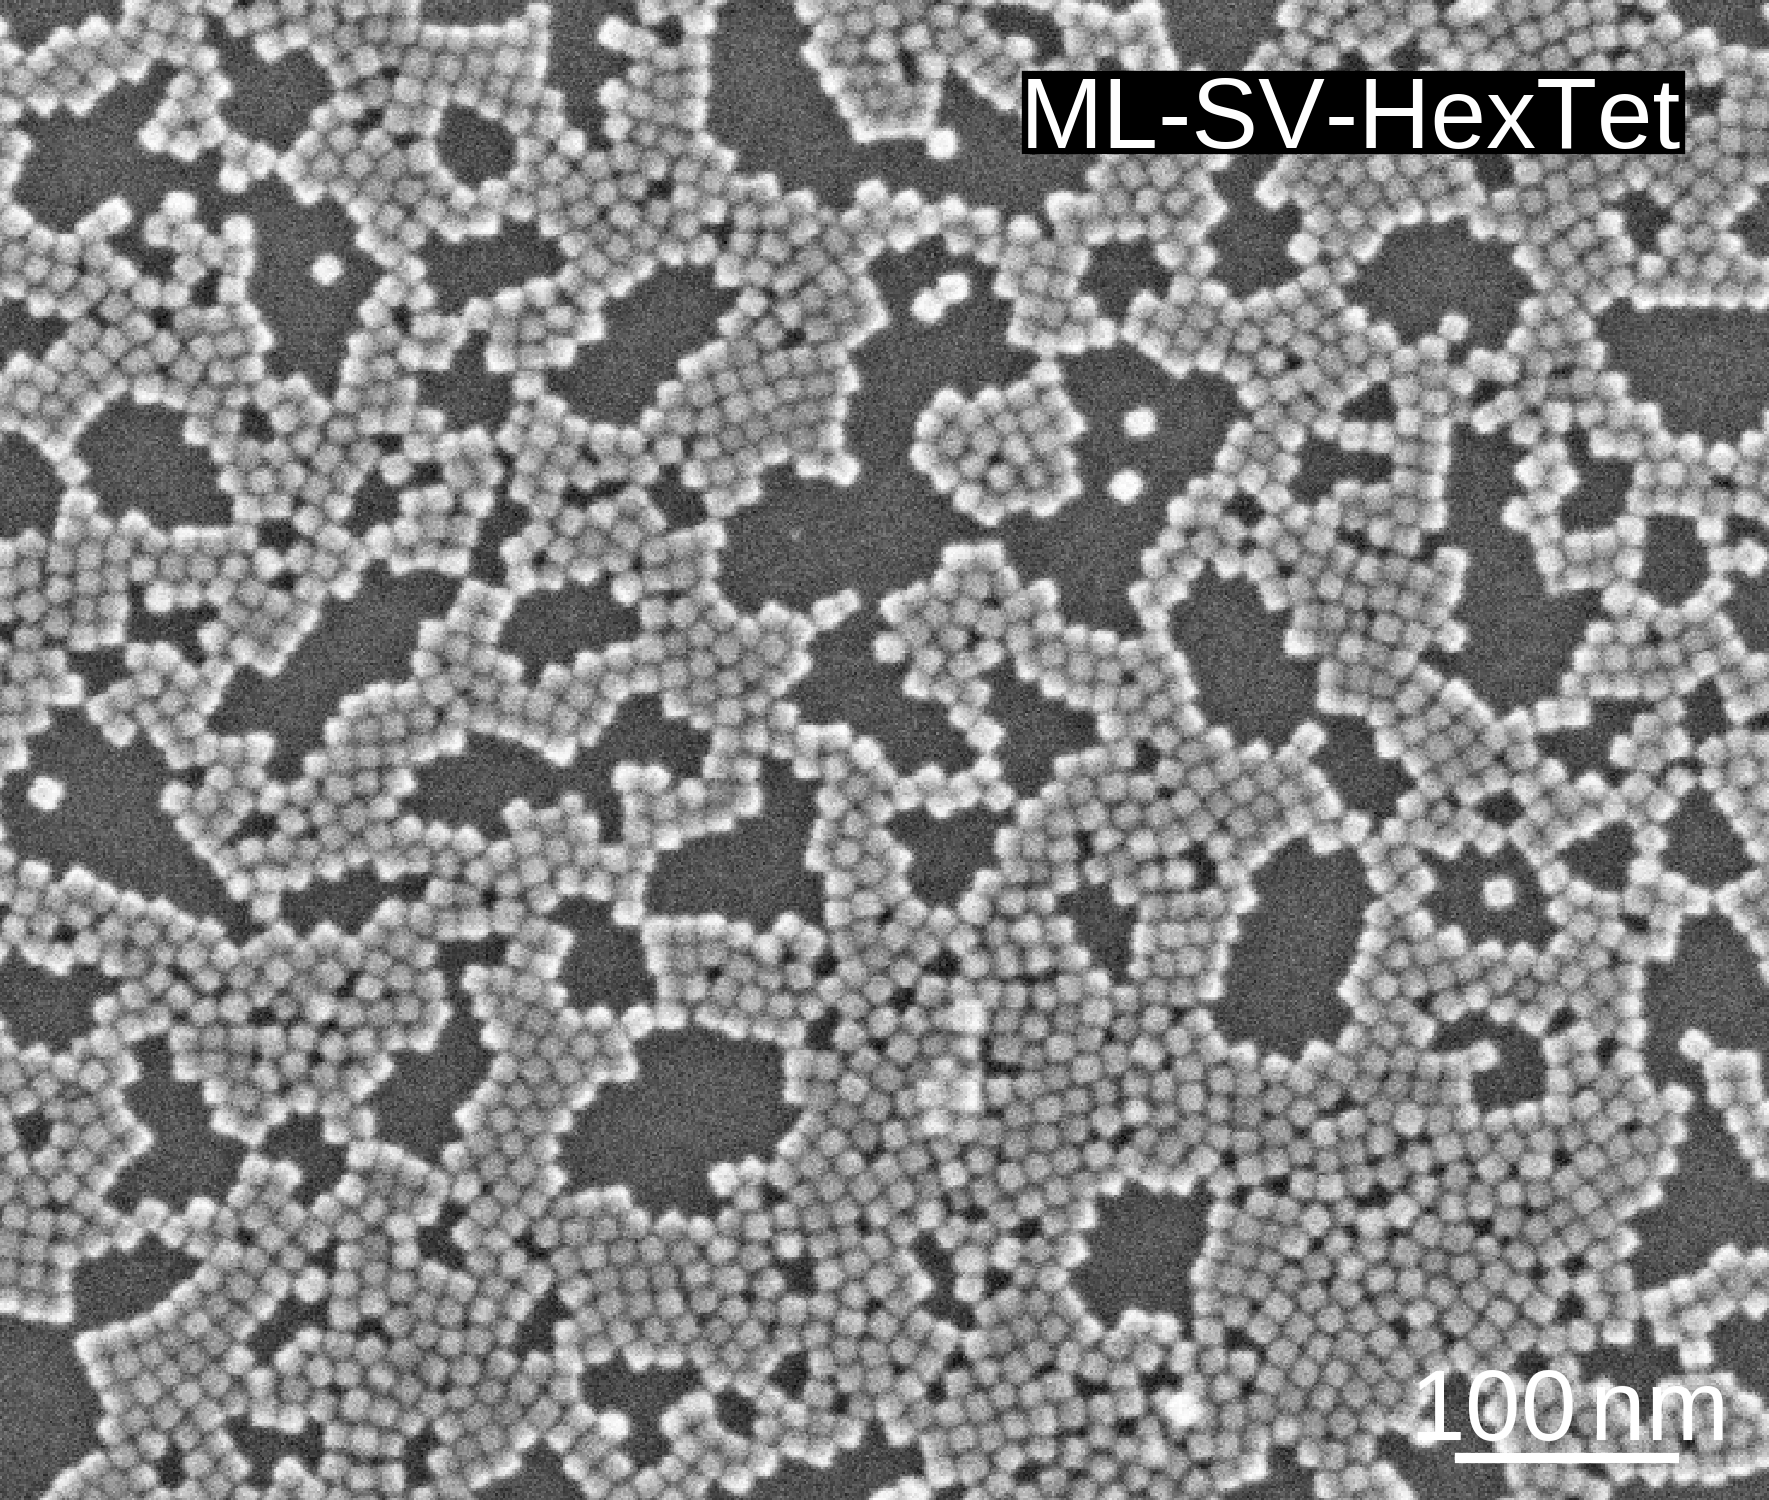
\includegraphics{monolayers_SEM_ML-SV-HexTet}
    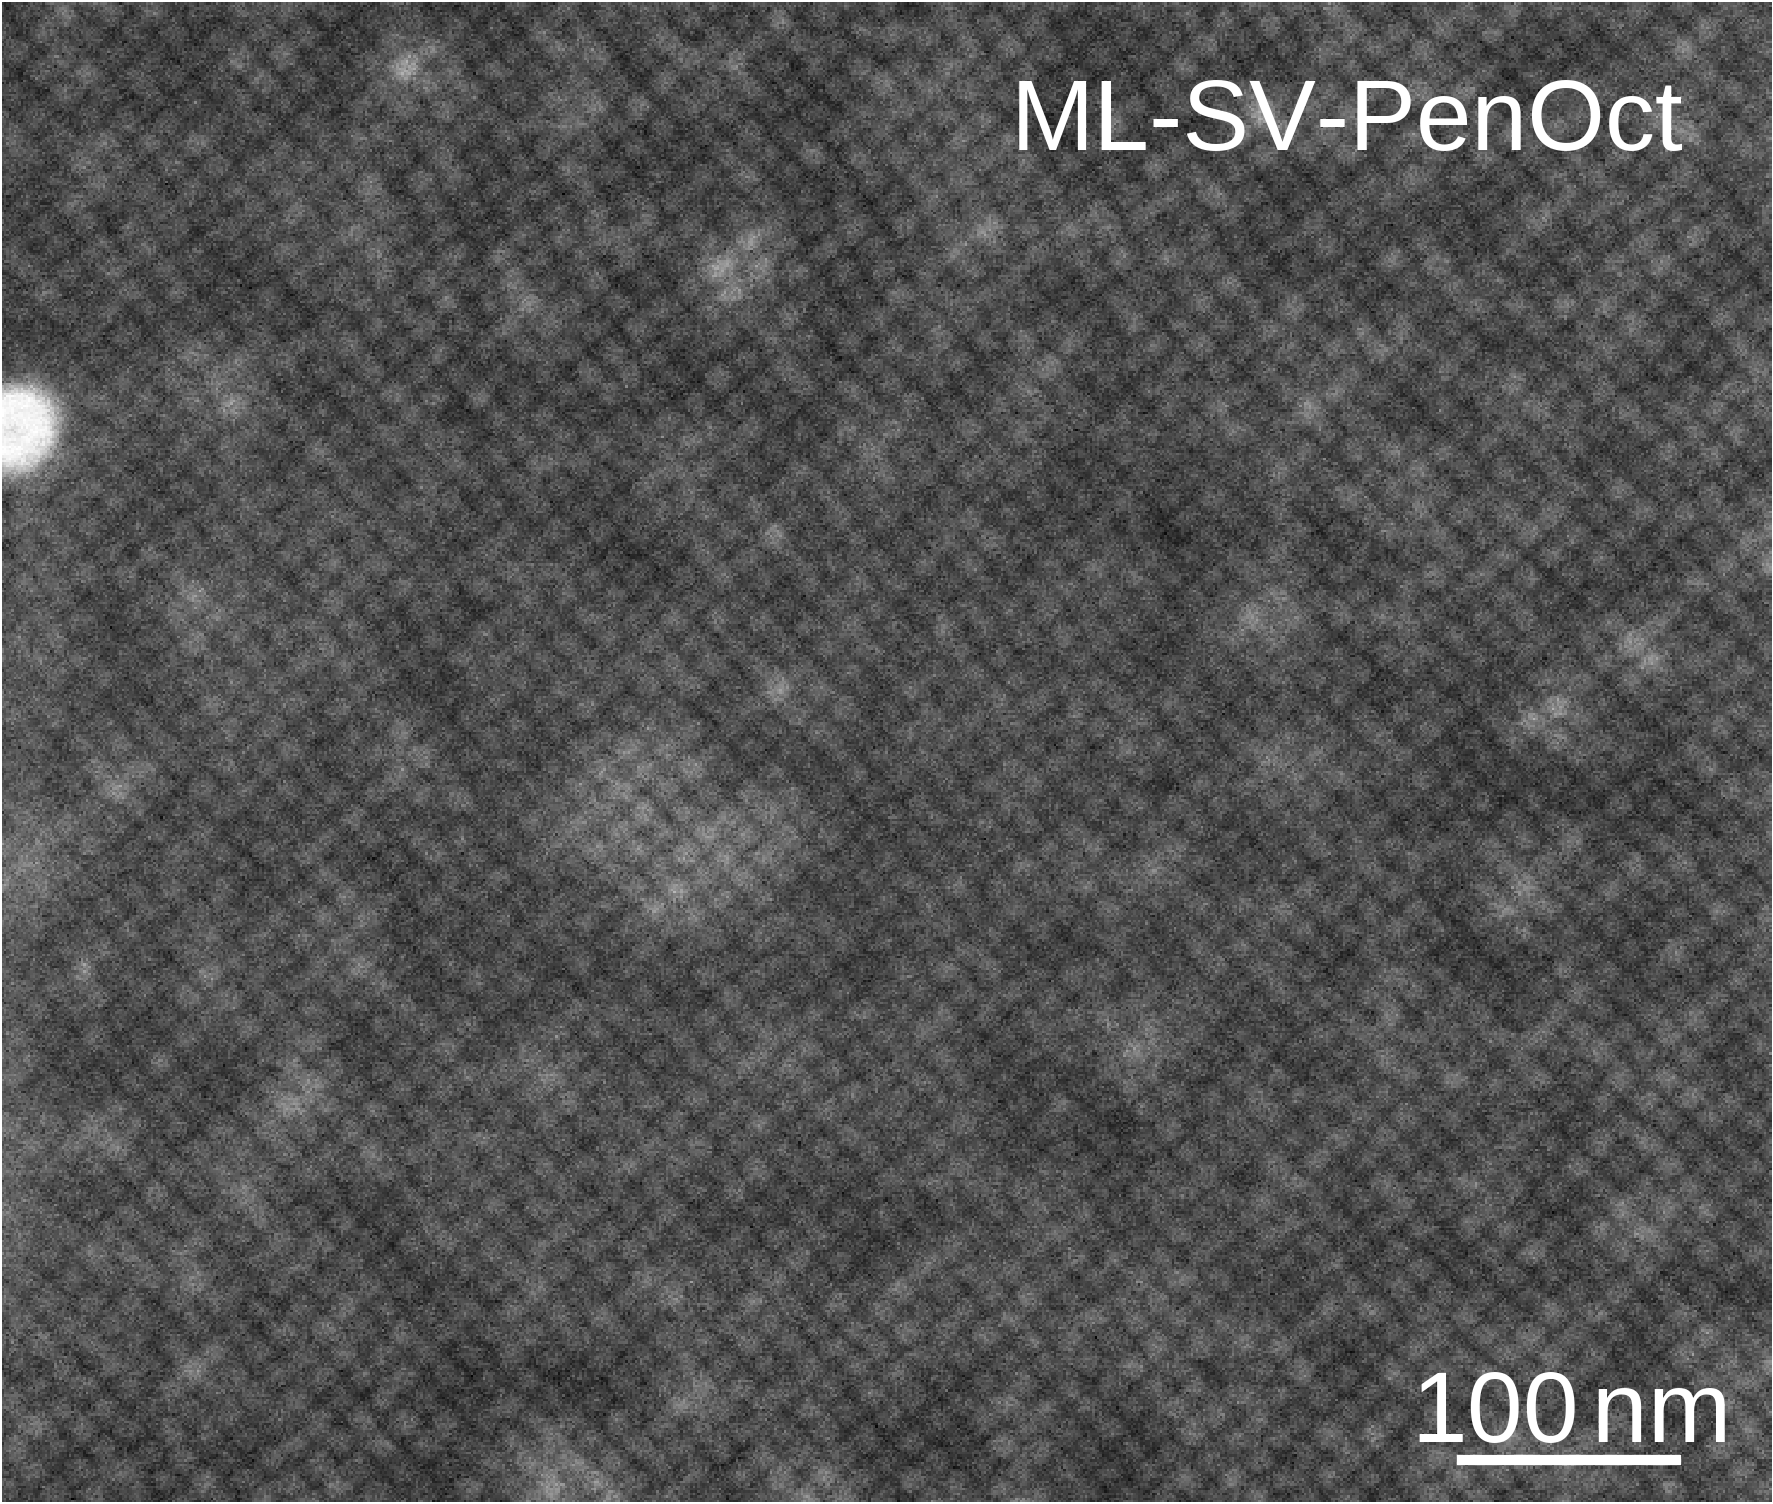
\includegraphics{monolayers_SEM_ML-SV-PenOct}
    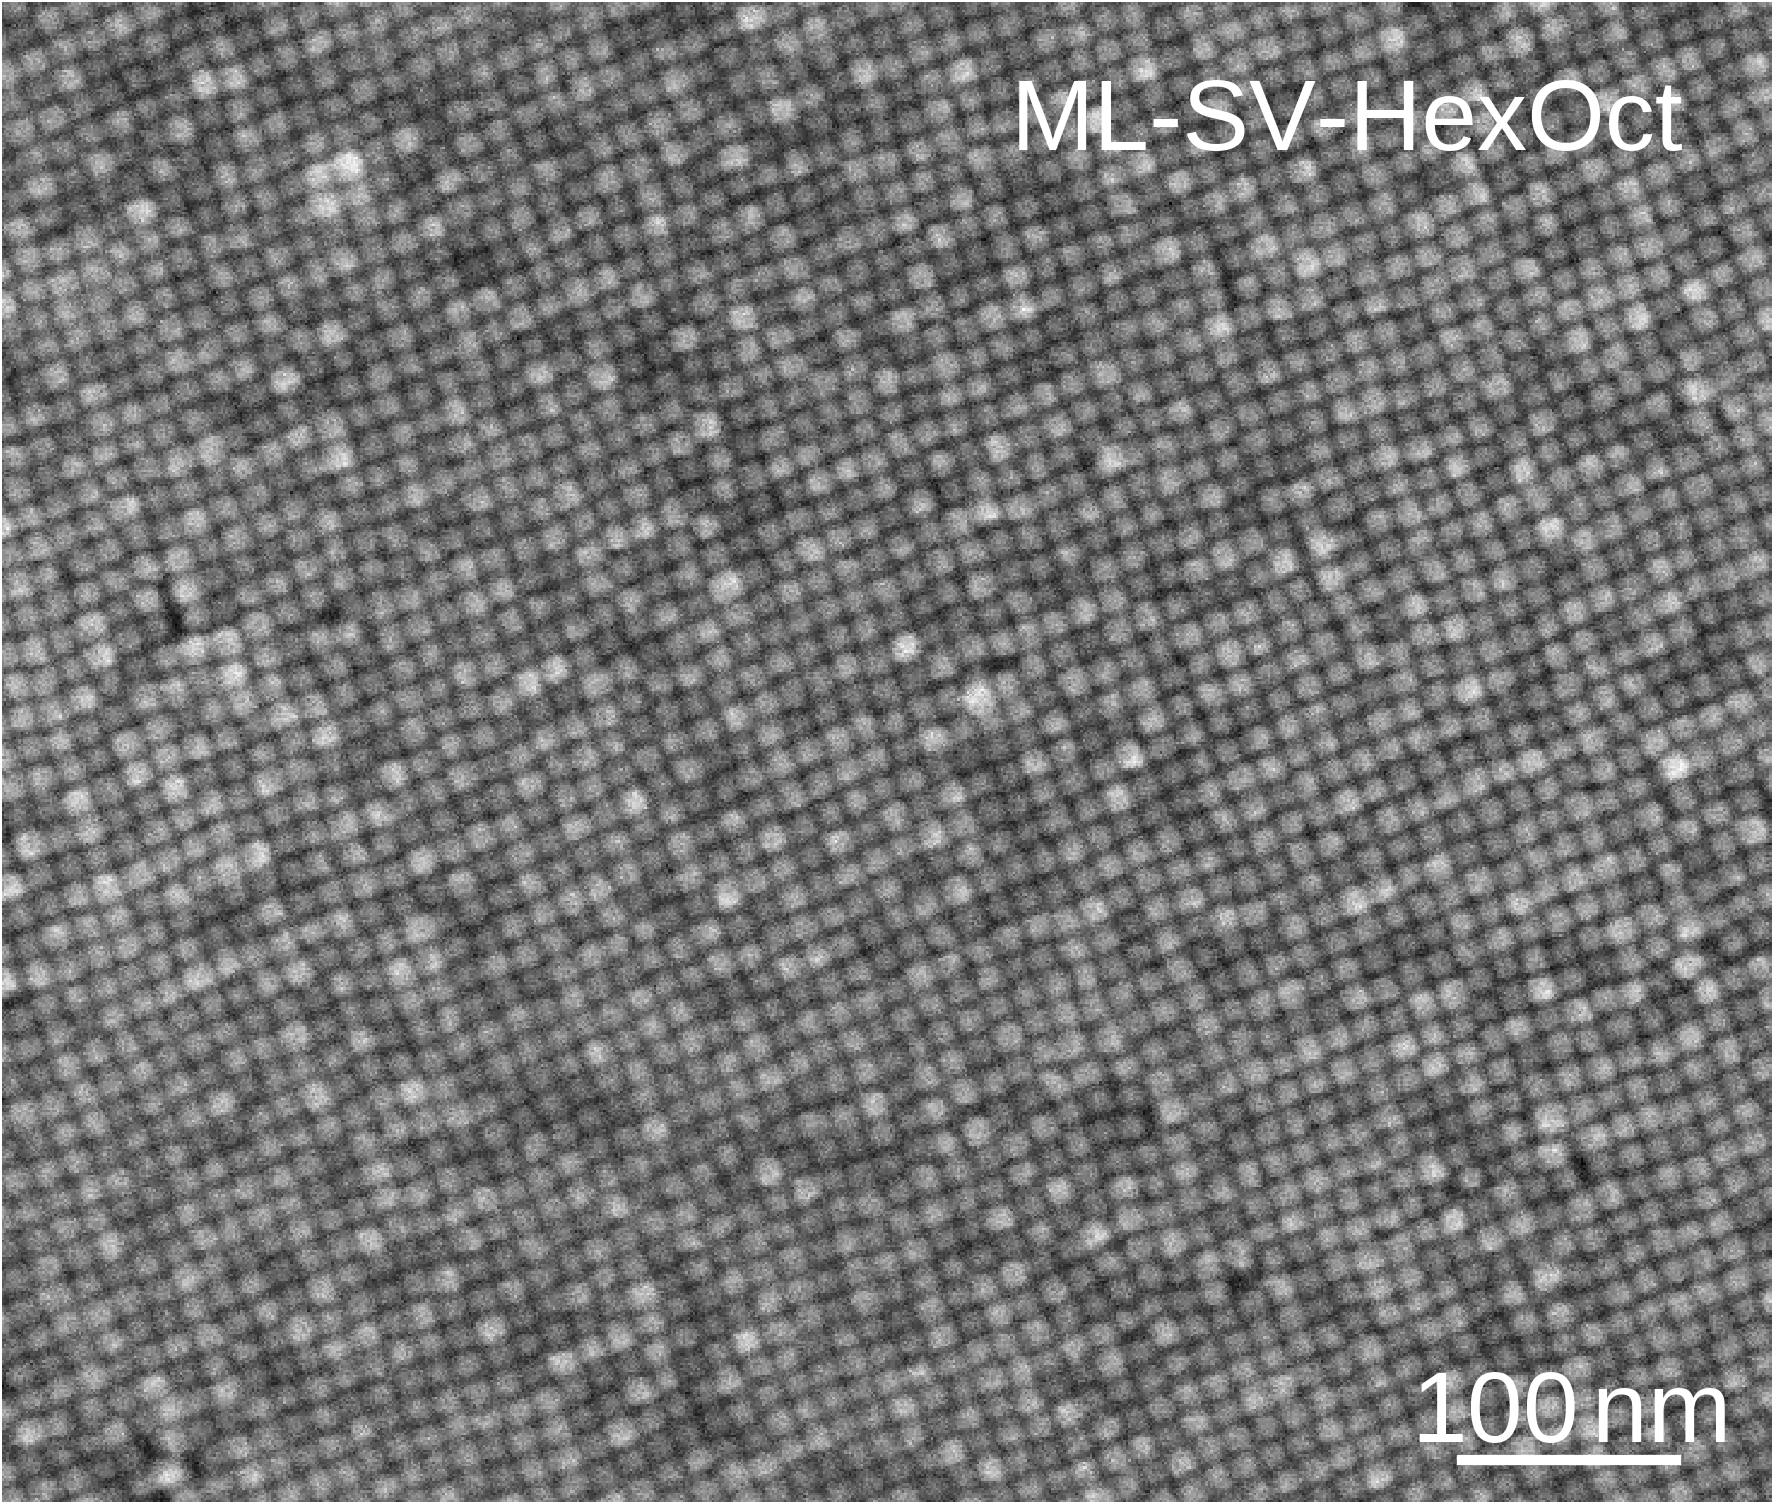
\includegraphics{monolayers_SEM_ML-SV-HexOct}
    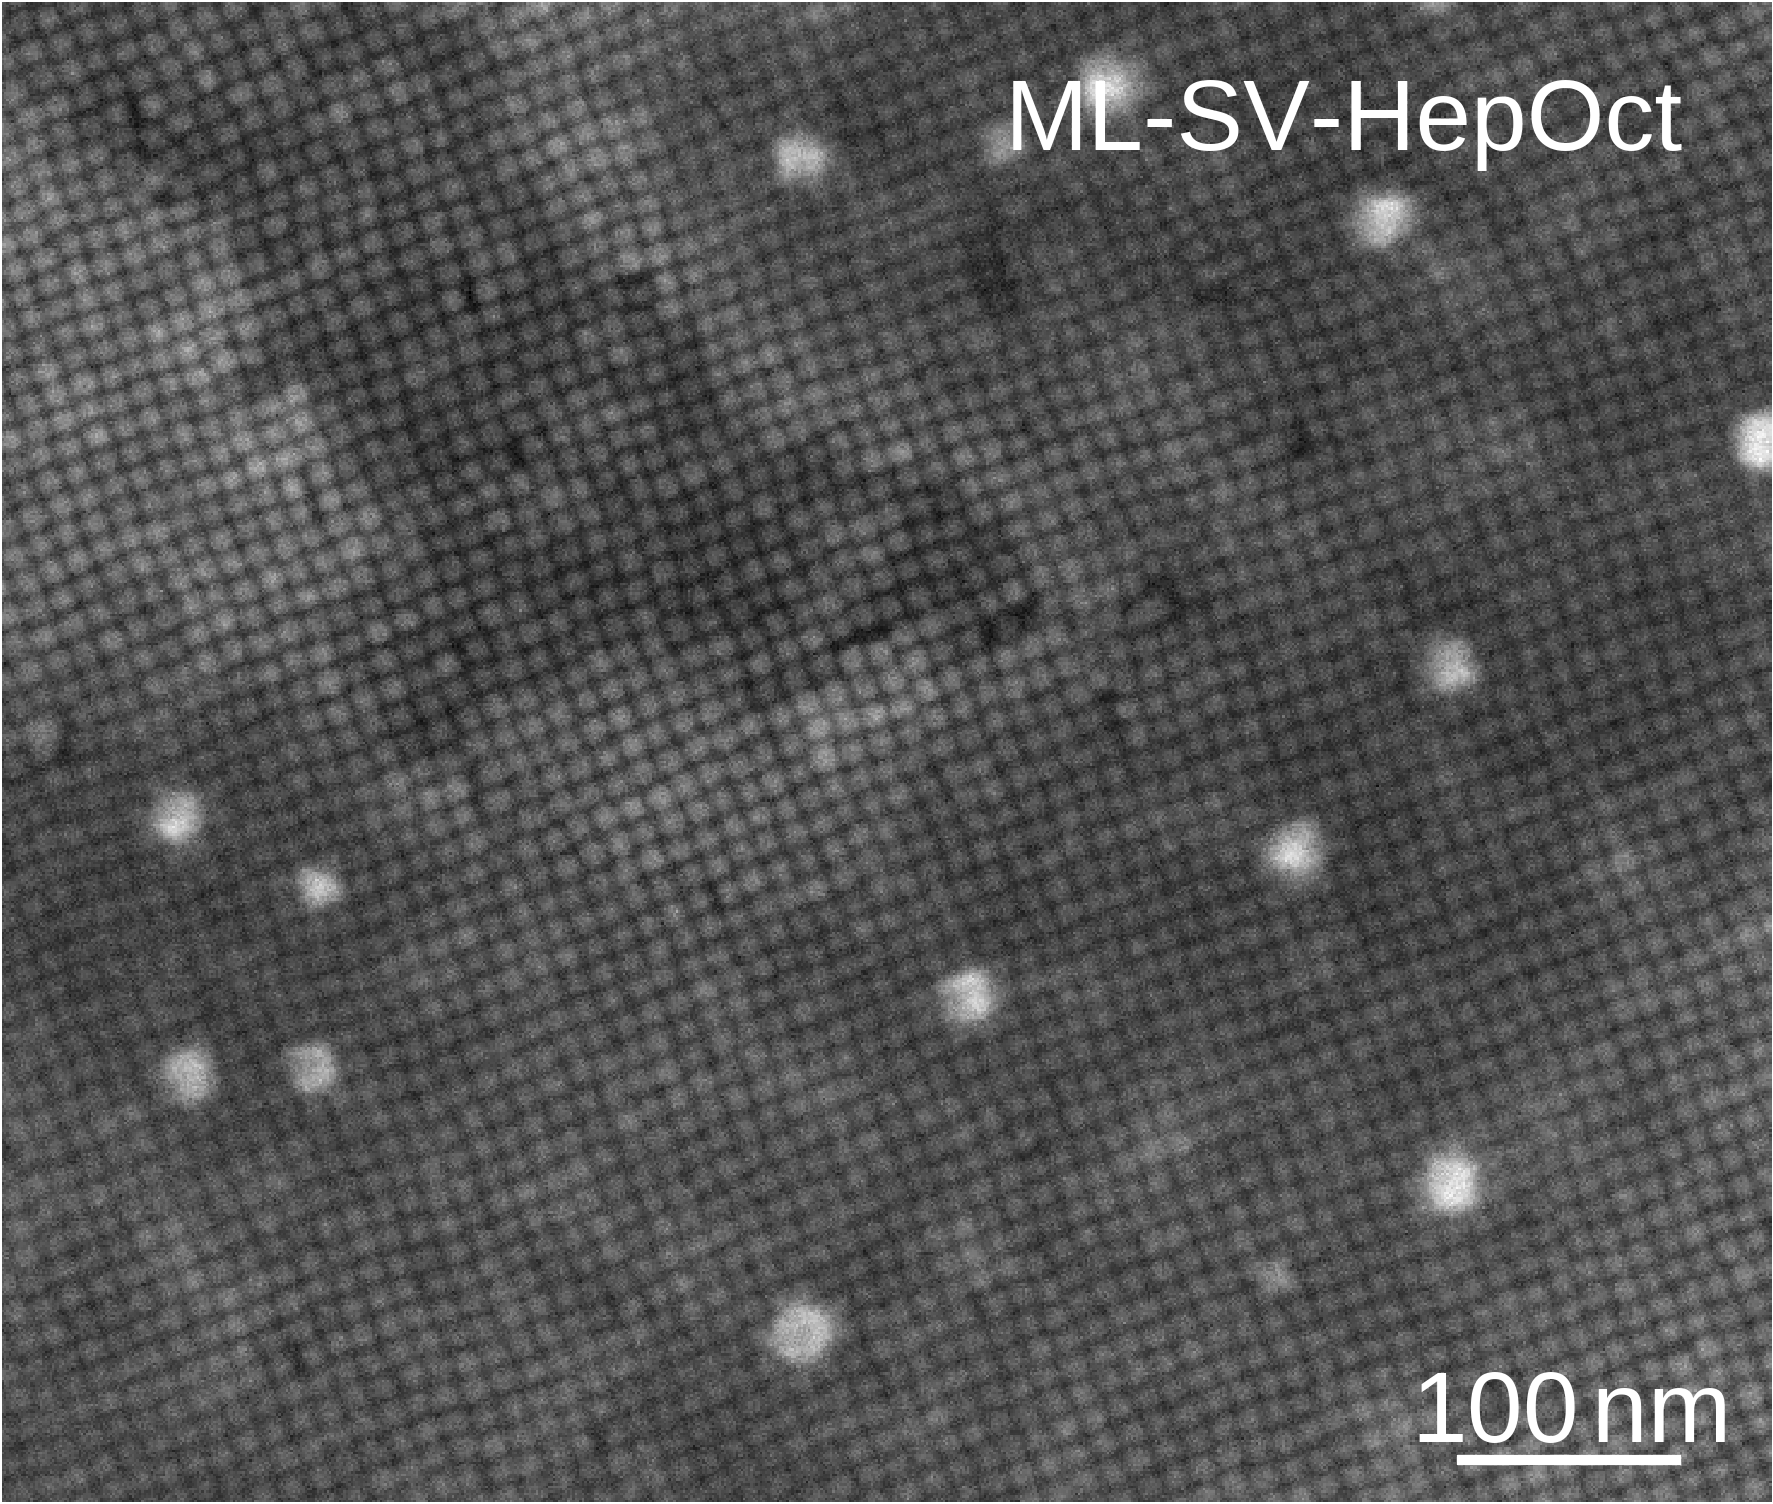
\includegraphics{monolayers_SEM_ML-SV-HepOct}
    \caption{\label{fig:monolayers:preparation:solventVariation:sem}Scanning electron microscopy of Ol-CoFe-C nanoparticles after drop casting using hexane/tetradecene (upper left),  pentane/octadecene (upper right), hexane/octadecene (lower left) and heptane/octadecene (lower right) as solvents.}
  \end{figure}

  Scanning electron microscopy is performed (\refapp{app:additionalExperimentalTechniques:sem}) for a first evaluation of the samples and to study the local order.
  In \reffig{fig:monolayers:preparation:solventVariation:sem} four exemplary samples of combinations are shown: A sample to show a combination of a alkene with a relatively low boiling point, 1-tetradecene, with n-hexane (ML-SV-HexTet), and three samples to show combinations of 1-octadecene with the varied alkanes n-pentane (ML-SV-PenOct), n-hexane (ML-SV-HexOct) and n-heptane (ML-SV-HepOct).
  ..Further combinations are given in App ??..
  A result that is imminently visible from SEM is that an alkene with a relatively low boiling point leads to no order formation. 
  Combinations with 1-octadecene however show for all alkanes local square order formation.
  For the variation of the alkane component, the local evaluation of SEM images shows only minor qualitative differences.

  \begin{figure}[tb]
    \centering
    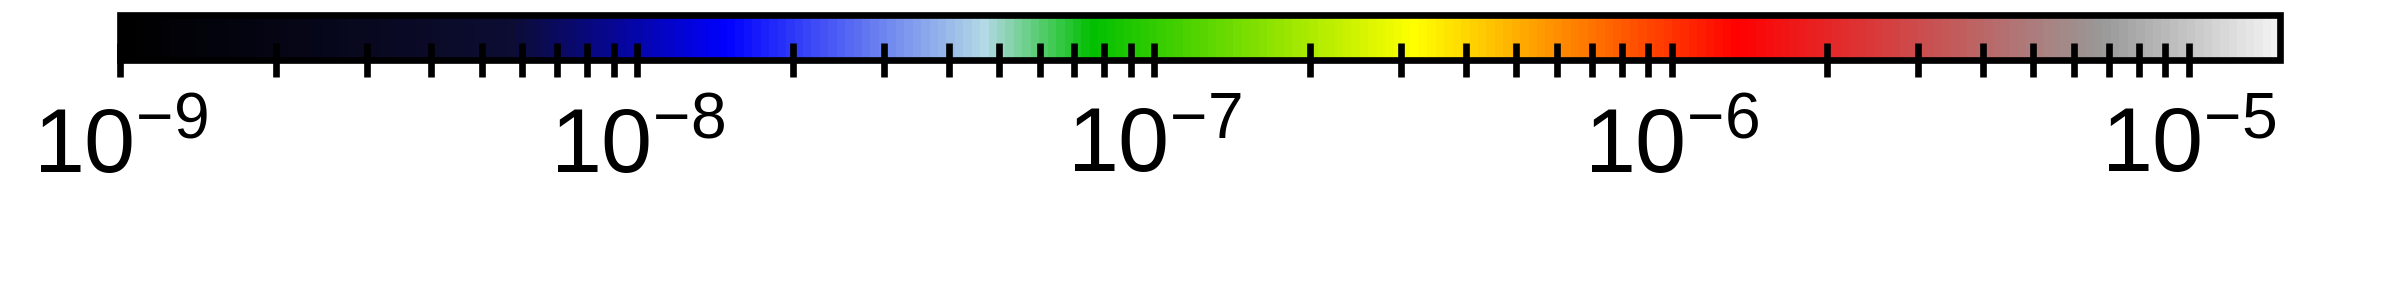
\includegraphics{monolayers_GISAXS_SVcbar}
    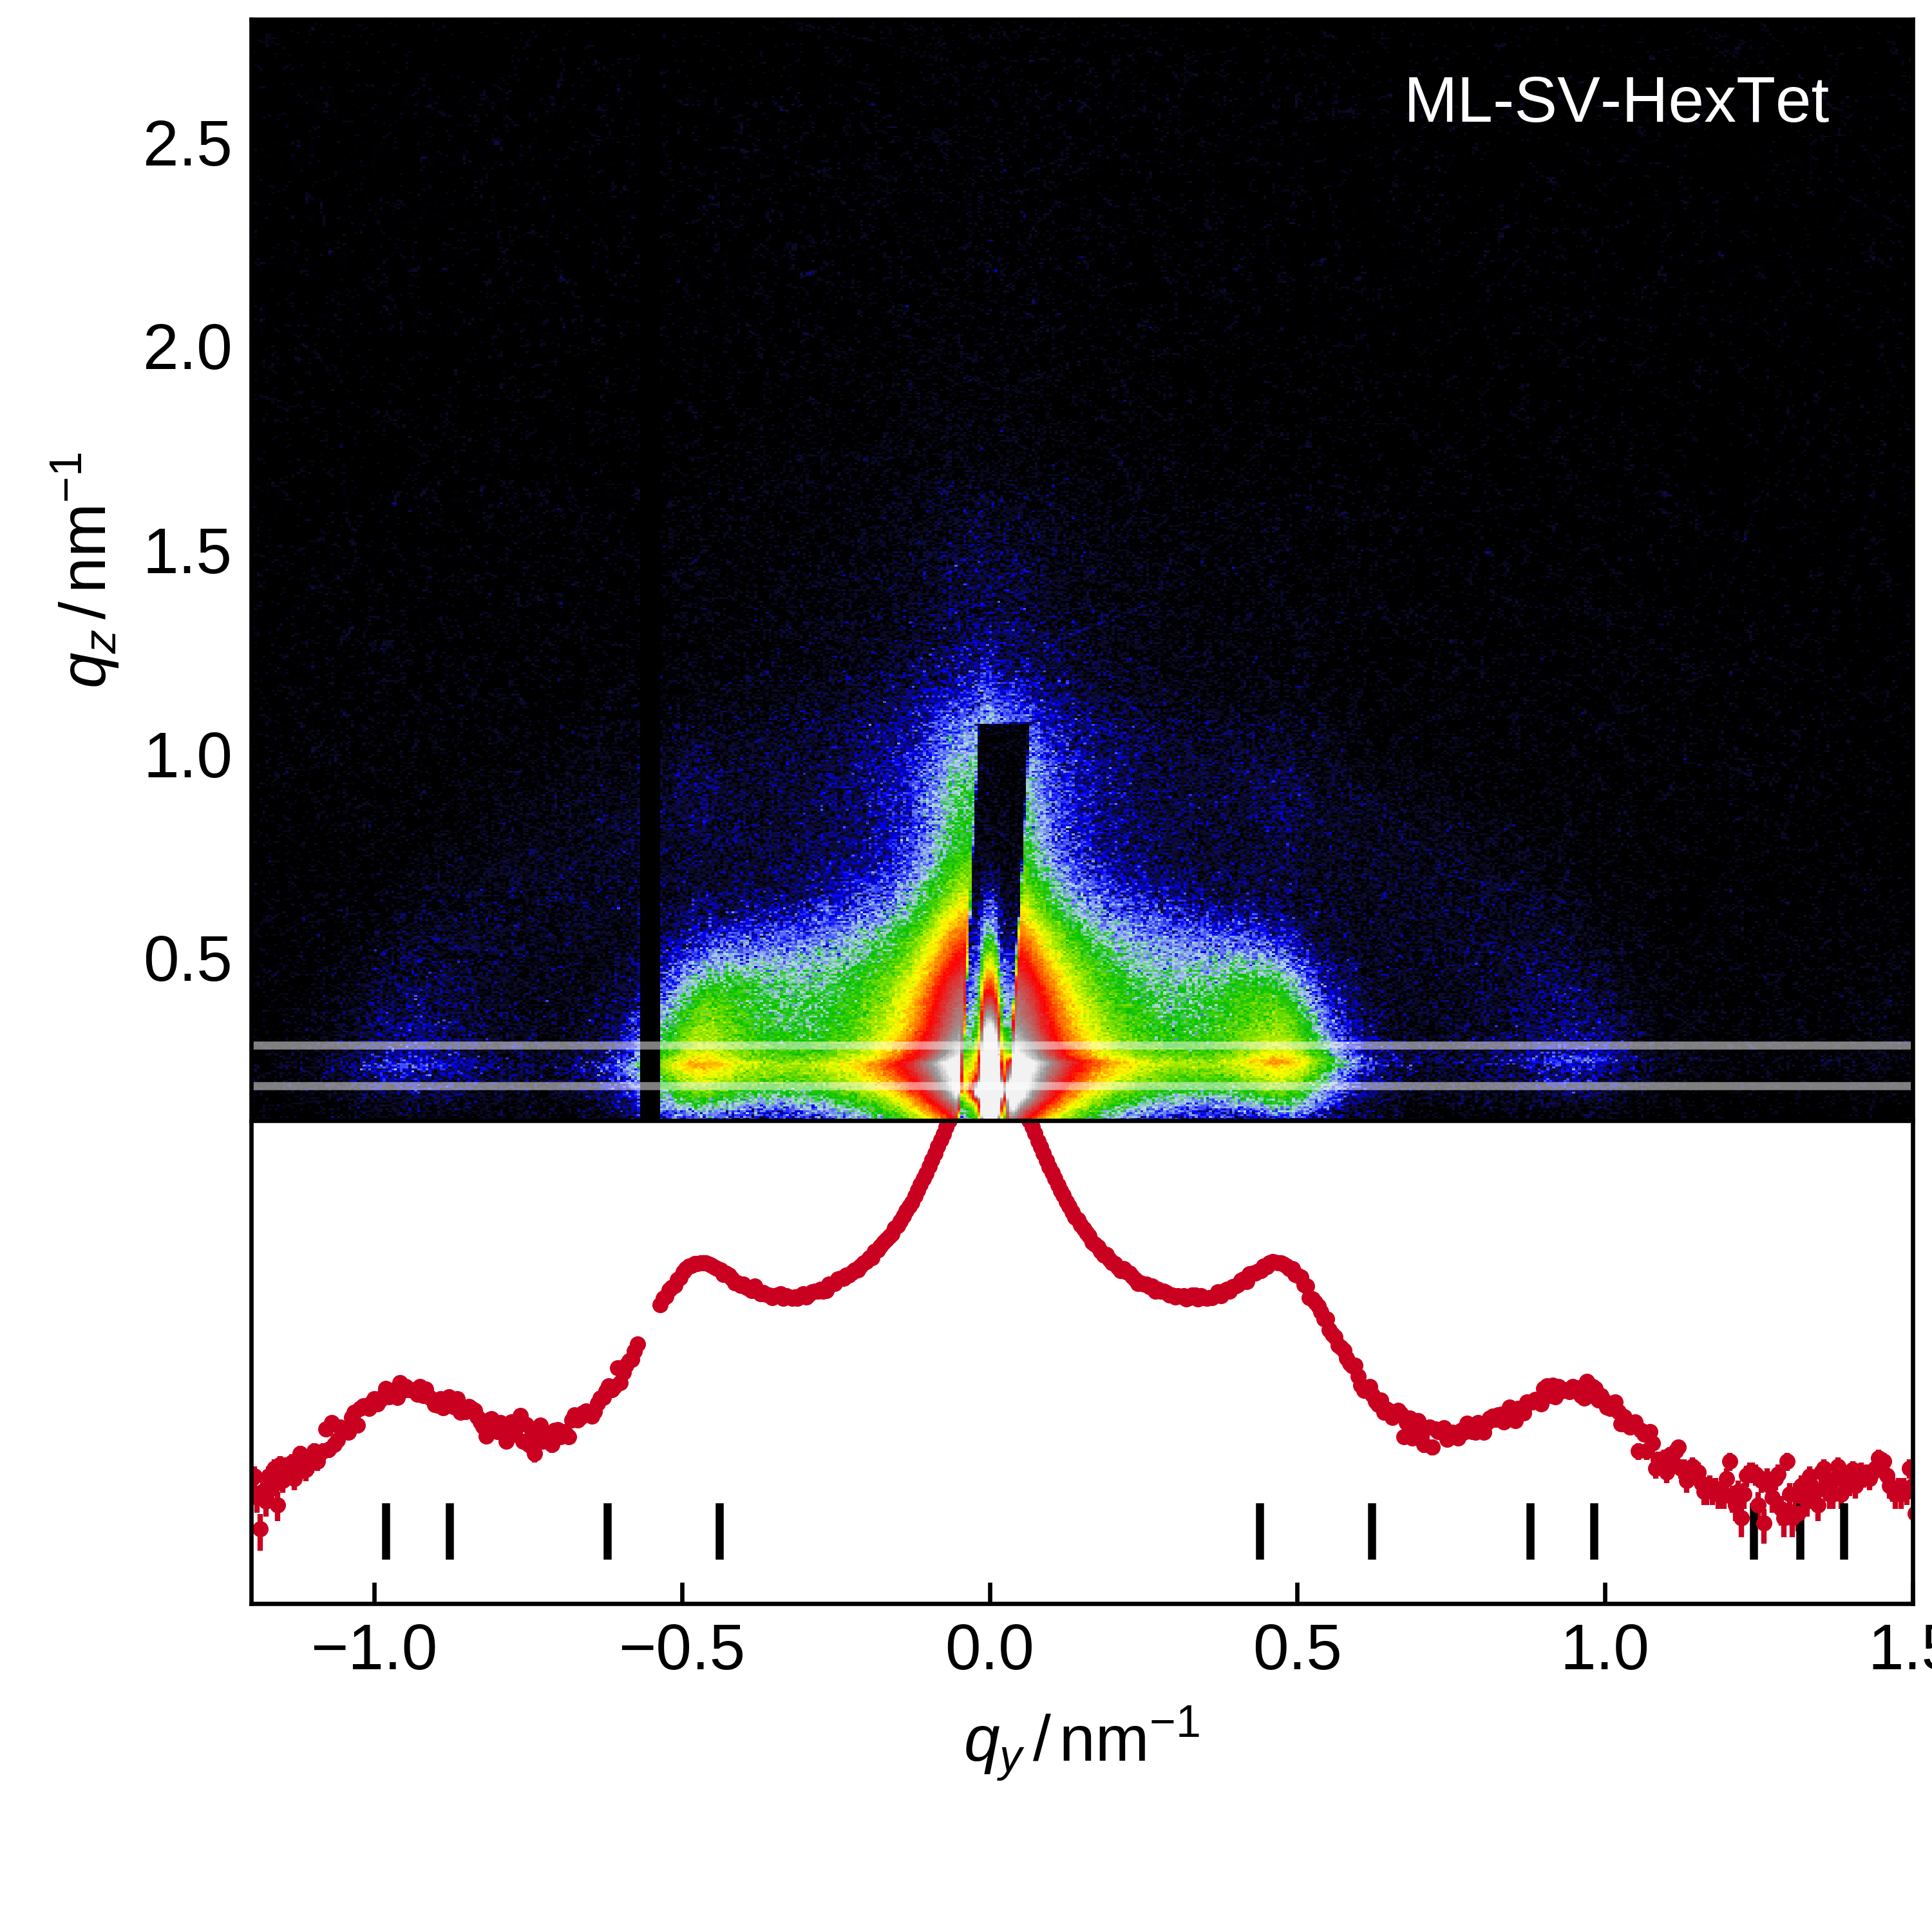
\includegraphics{monolayers_GISAXS_ML-SV-HexTet}
    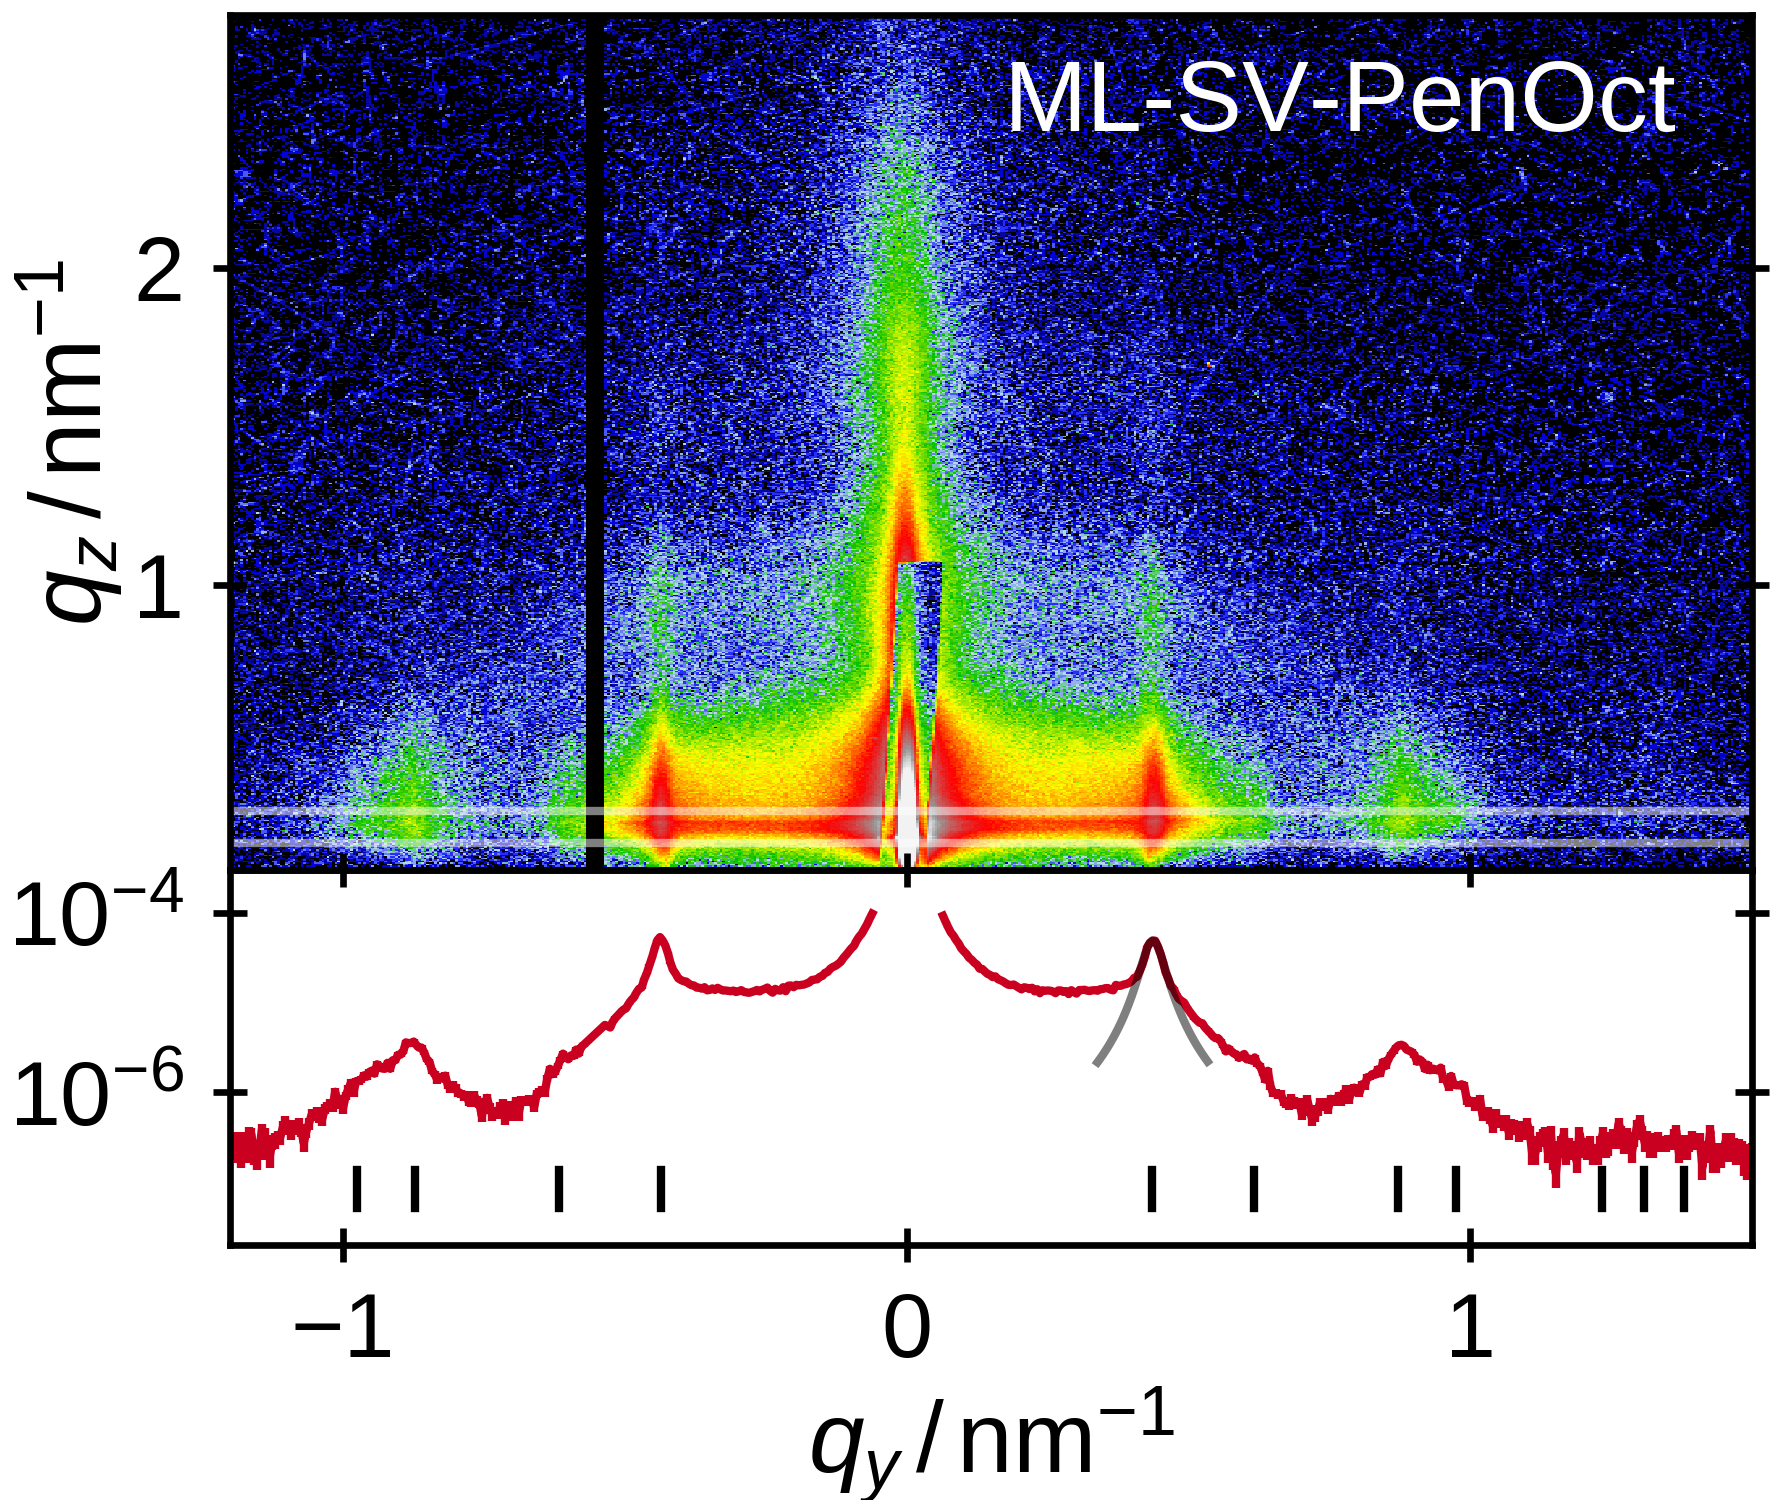
\includegraphics{monolayers_GISAXS_ML-SV-PenOct}
    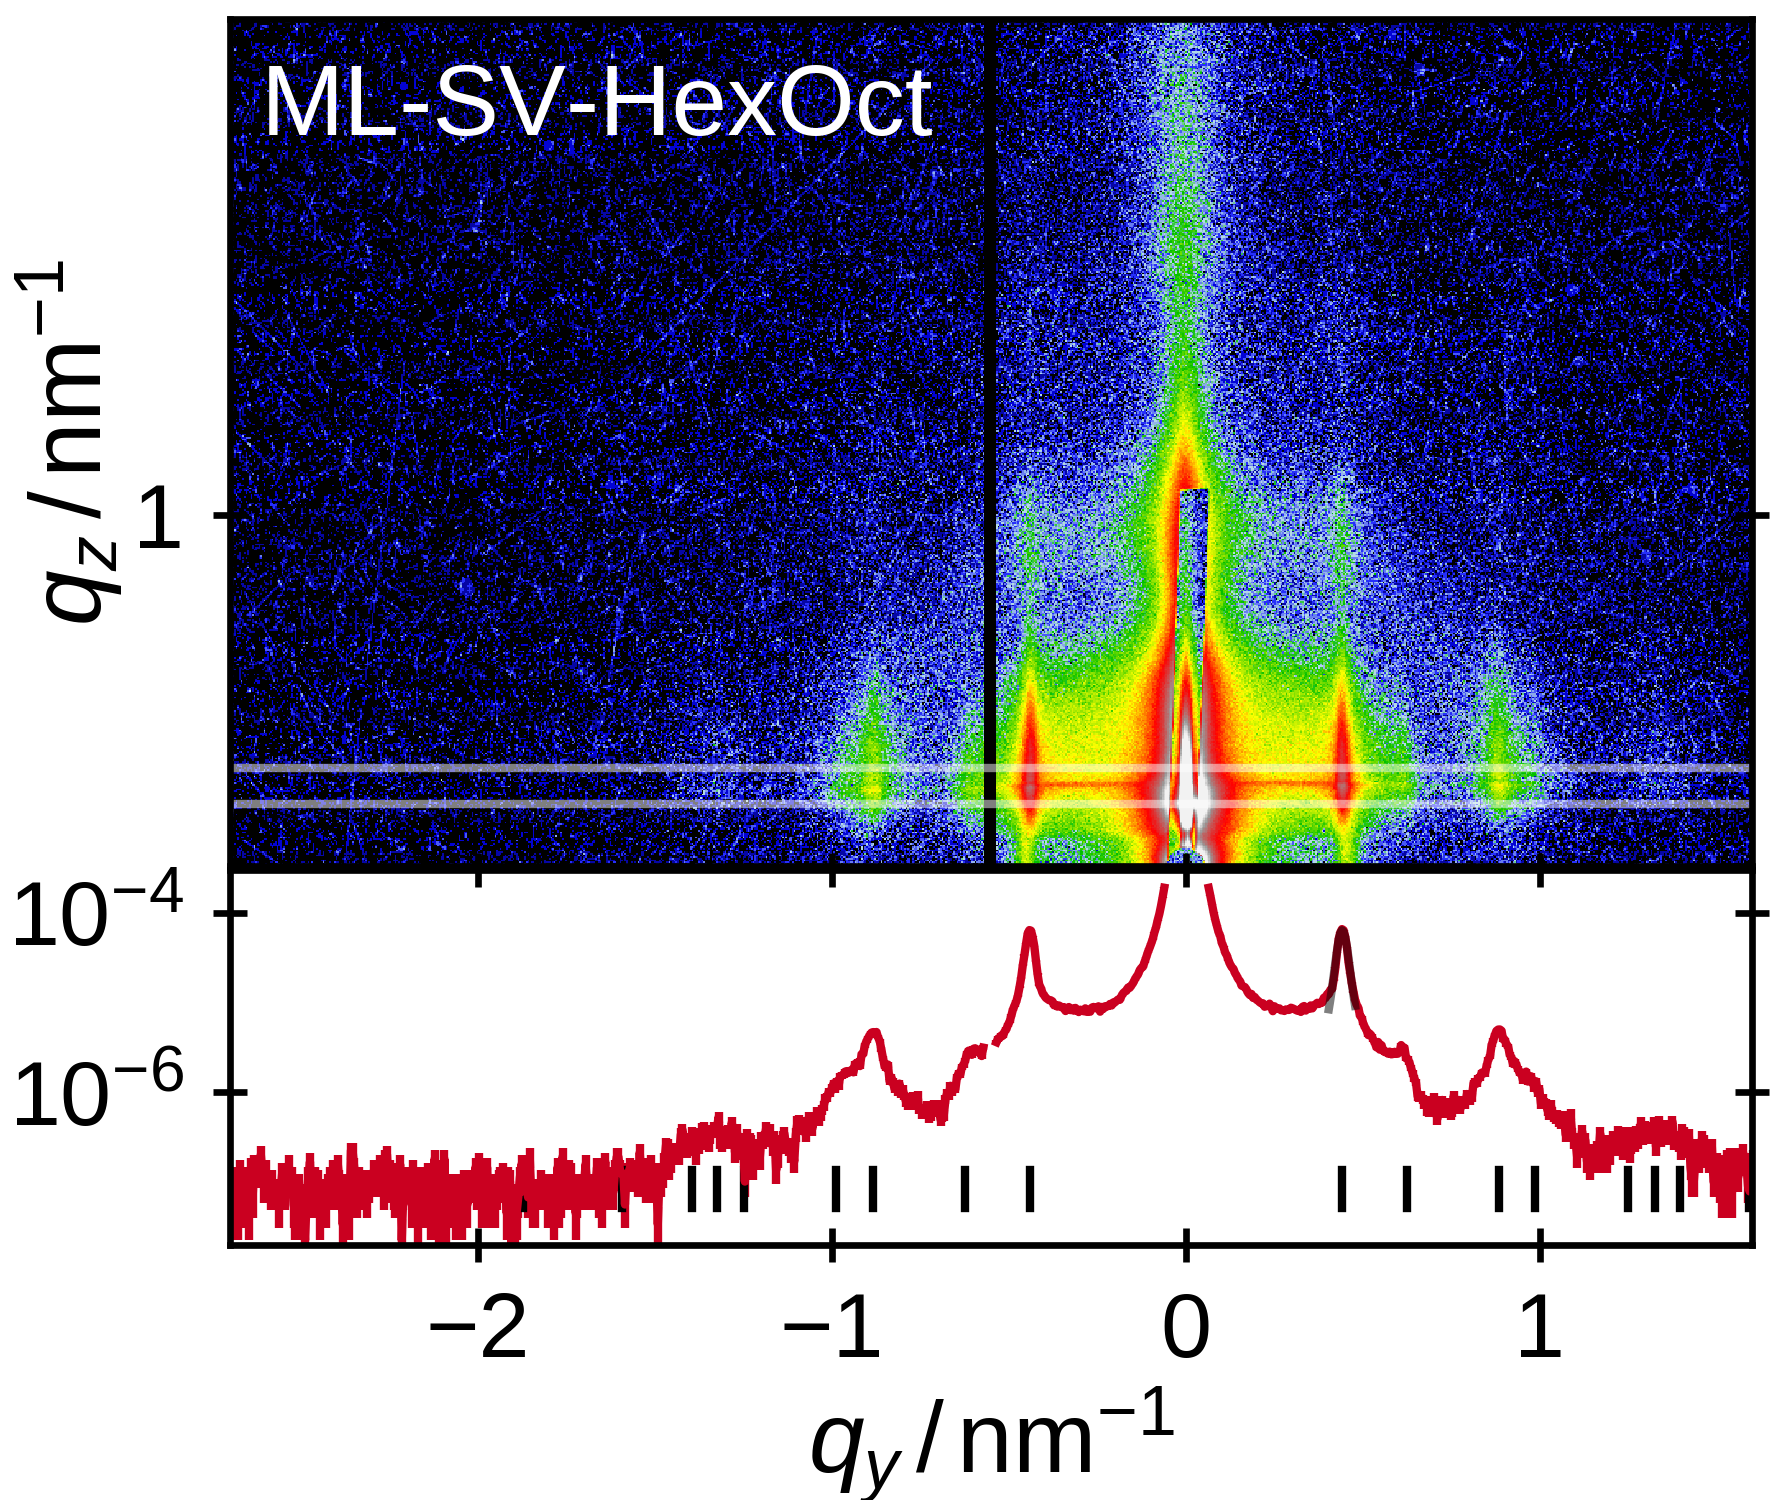
\includegraphics{monolayers_GISAXS_ML-SV-HexOct}
    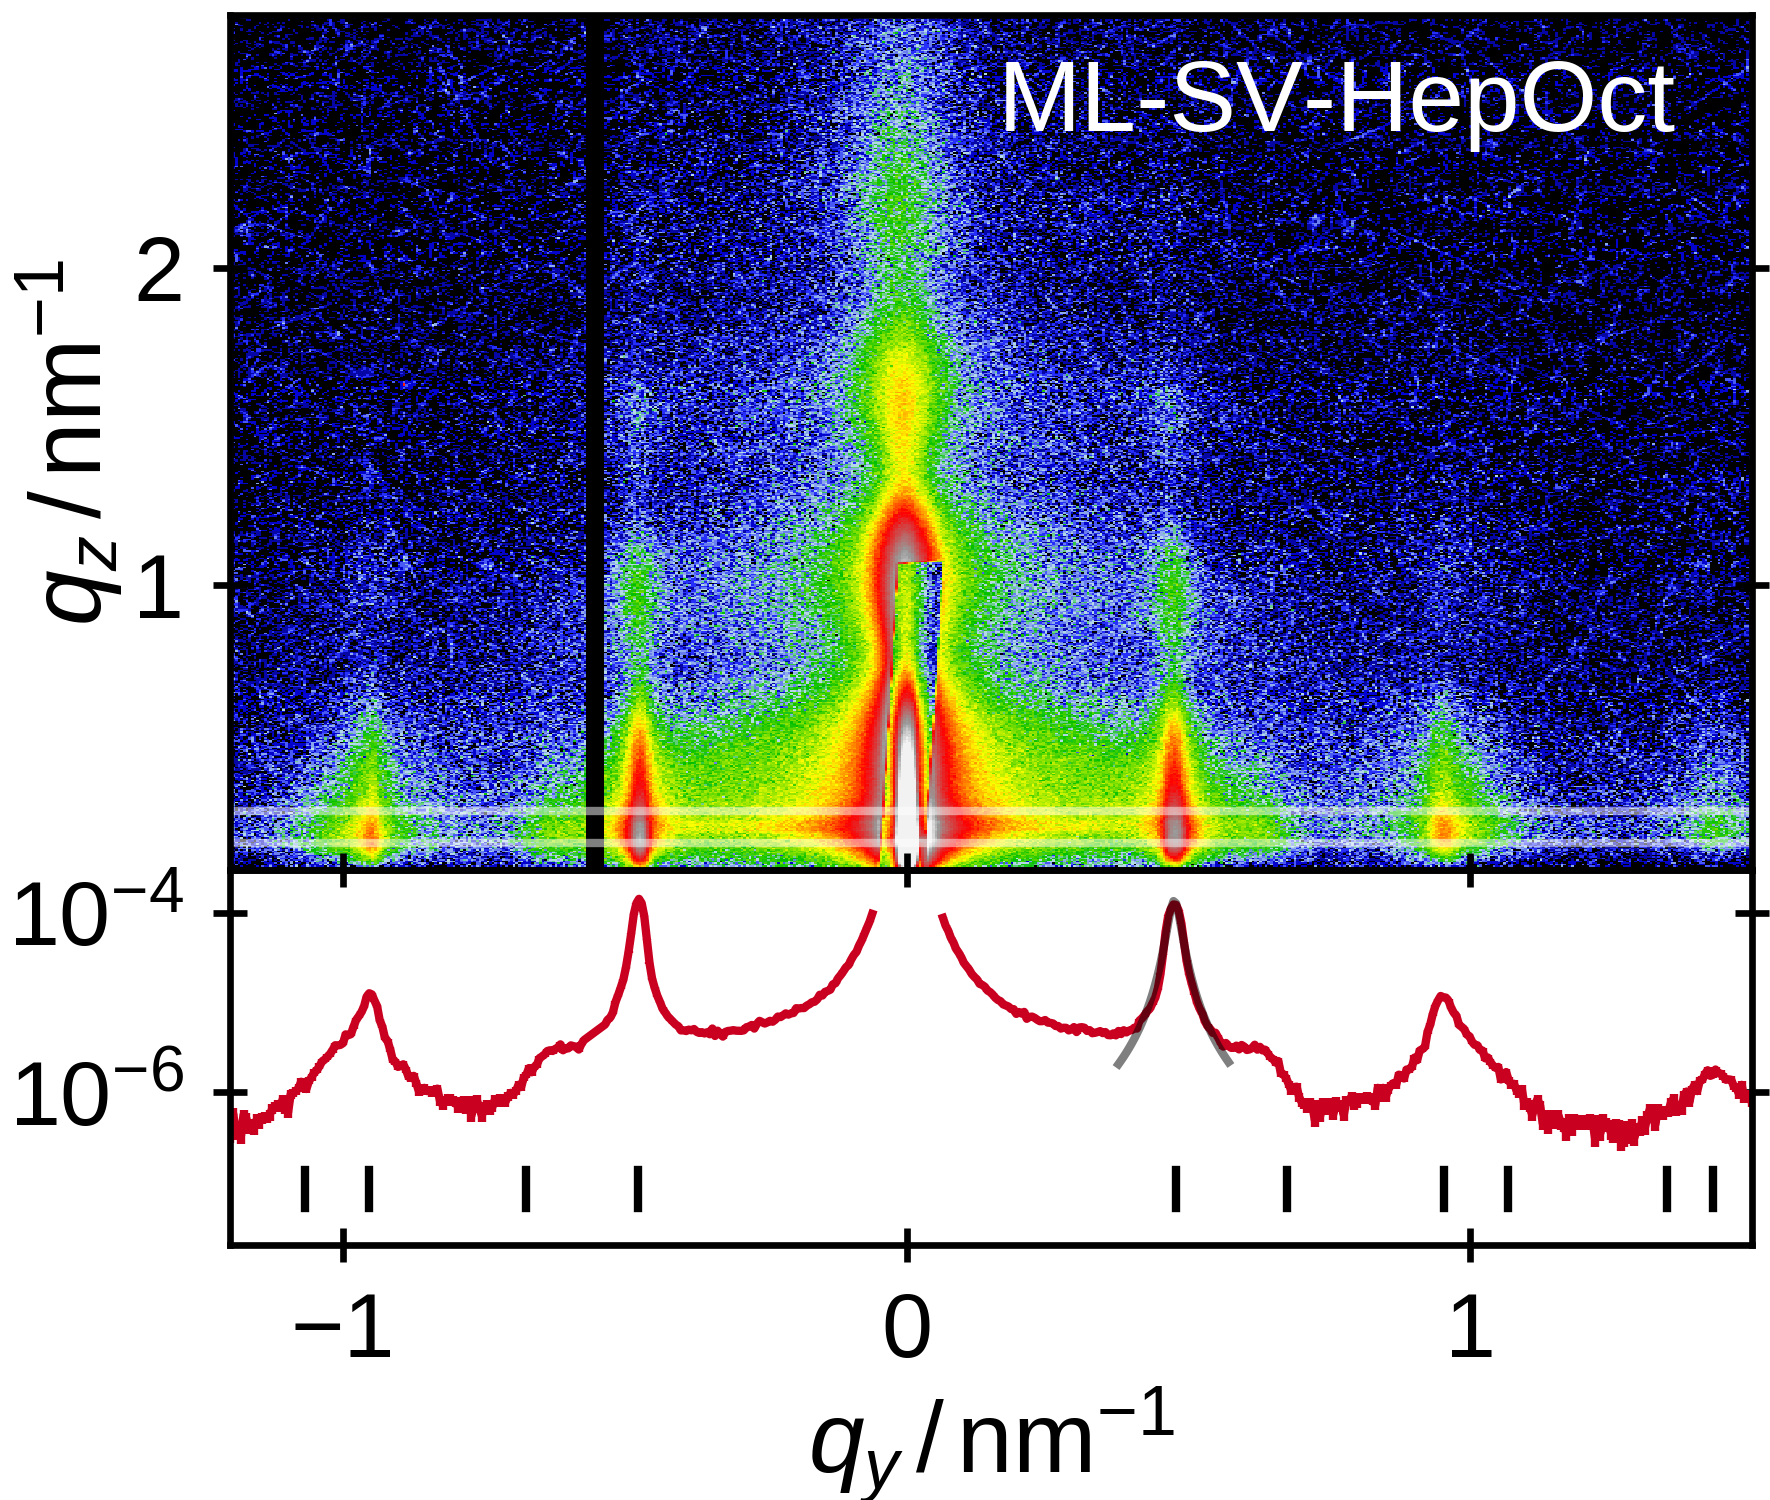
\includegraphics{monolayers_GISAXS_ML-SV-HepOct}
    \caption{\label{fig:monolayers:preparation:solventVariation:gisaxs}GISAXS detector images to study the average lateral structure globally for the same samples as shown in \reffig{fig:monolayers:preparation:solventVariation:sem}. Below the detector images, the intensity in a stripe around the Yoneda line  }
  \end{figure}
  Thus to quantify the in-plane order, the selected samples are measured using grazing incidence small-angle x-ray scattering at GALAXI (\refapp{ch:appendix:lss:galaxi}) under an incident angle of $\alpha_i \eq 0.11 \unit{^\circ}$.
  The resulting detector images are shown in \reffig{fig:monolayers:preparation:solventVariation:gisaxs}.
  Similar to SEM, ML-SV-HexTet shows no significant structure factor along the Yoneda line, but mainly scattering coming from the form factor of the individual nanoparticles.
  For the other three shown samples, higher order alkanes show the emergence of structure peaks.
  The peak positions are compared to the expected relative positions for a square lattice, given by
  \begin{align}
    q_{hk} \eq \frac{2 \pi}{a} \sqrt{h^2 + k^2},
  \end{align}
  where $h$, $k$ are integers and $a$ the lattice constant of the square arrangement.
  To quantify the thin layer structure, x-ray reflectometry is performed at a Bruker D8 instrument (\refapp{app:additionalExperimentalTechniques:xrr}) where the incident angle is varied in the range of $0\unit{^\circ} - 2\unit{^\circ}$.

  The best quality of samples is achieved for a combination of n-heptane together with small addends of 1-octadecene and oleic acid as co-solvents.


  A more detailed investigations of the various combinations
  ...appendix..
  shows that, while combinations with 1-hexadecene still give rise to some short range order, only combinations with 1-octadecene lead to long range order across several micrometers.


\end{document}